%*******************************************************
% System Architecture
%*******************************************************
\pdfbookmark[1]{System Architecture}{System Architecture}
\chapter{System Architecture}

\section{Introduction}
This document details the general system architecture design of FollowThrough. It goes in to detail on the major decisions that were made at key points throughout the product. It also discusses the changes that are likely and unlikely. Lastly it mentions how the requirements are linked to the design.

\subsection{Terms Used}
\begin{table}[h!]
  \centering
  \caption{Terms Used}
  \label{tab:table2}
  \begin{tabular}{ccc}
    \toprule
    Term & Description\\
    \midrule
    FollowThrough & The name of the product.\\
    Arduino & The processor for the hardware used.\\
    Form & Refers to the user's shot form in Basketball.\\
    \bottomrule
  \end{tabular}
\end{table}

\subsection{Tables Used}
\begin{table}[h!]
  \centering
  \caption{List of Tables}
  \label{tab:table3}
  \begin{tabular}{ccc}
    \toprule
    Number & Name\\
    \midrule
    2 & Terms Used\\
    3 & List of Tables\\
    4 & List of Figures\\
    5 & Pro/Con Chart\\
    6 & Traceability Chart\\
    \bottomrule
  \end{tabular}
\end{table}

\newpage
\subsection{Figures Used}
\begin{table}[h!]
  \centering
  \caption{List of Figures}
  \label{tab:table4}
  \begin{tabular}{ccc}
    \toprule
    Number & Name\\
    \midrule
    1 & Uses Hierarchy\\
    \bottomrule
  \end{tabular}
\end{table}

\section{Overview}

\subsection{Purpose of the Project}
This product is to be used by the common Basketball player so that they may improve their form without having to go through the expenses of a personal coach. FollowThrough is an inexpensive tool which provides the user real time feedback while they are on a Basketball court.

\subsection{General Description}
As mentioned previously this product gives the user real time feedback so that they may improve their form. The data gathered on site is recorded and then sent to an on line database. The user may afterwards review all the gathered data through an on line interface. This will maximise the potential for improving the user's form. To preface the rest of this document, the architecture style we have chosen for our product is largely client-server.

\subsection{Document Structure}
This document was separated into two sections; the first being System Architecture and the other being Component Design.

\section{Important Design Decisions}

\subsection{The Online Interface}
This portion of the product was included because we realised that a user would very likely want to review all their data on another date. While receiving real time feedback is the main point of the product, in some cases the information can be overwhelming. This is where the on line interface comes in to play. On top of that there would be no reason to memorise what needs to be changed in the user's form, because it's all on line. This only takes work off of the user and makes the product more convenient.

\subsection{Databases}
The tables that the server will hold will be as follows: A user table and a shot table. The user table contains a user ID (Primary Key), a user name (Unique), an email (Unique), a password, a first name and a last name. The shot table will contain a shot ID, date the shot was made, user ID (Foreign Key) and data on each shot such as location it was taken, distance from the net, over or under shot, details of the arc and if the shot was made or missed. The tables will have a one to many relationship from users to shots. This will ensure that the system is scalable and none of the information is missed.

\subsection{Haar Cascade Files}
A major issue addressed at the beginning of this project is having an effective way to track the ball. We decided to use Haar cascade files to solve this issue. A Haar cascade file is a file which compiles all the features of an object by putting together many images of that object. This accounts for colour, texture, lighting, shape... etc. The cascade file will take a long time to compile, so it will be compiled ahead of time, prior to launch. The other options were to simply track by colour, shape or size. All the options were outlined below in the Pro/Con chart.\\

\begin{table}[h!]
  \centering
  \caption{Pro/Con Chart}
  \label{tab:table5}
  \begin{tabular}{ccc}
    \toprule
    Method & Pros & Cons\\
    \midrule
    Size Tracking & Simple to implement, fast to run. & Cannot account for depth.\\
    Color Tracking & Simple to implement, fast to run. & Cannot account for background objects.\\
    Shape Tracking & Simple to implement, fast to run. & Cannot account for depth.\\
    Haar Cascade & Removes all noise. & Takes a long time to create.\\
    \bottomrule
  \end{tabular}
\end{table}

Regardless of the fact that all other options were simpler to implement and quite fast to run on hardware, background noise was a big problem with them all. Haar cascade files were chosen because it removes noise, and the only con is remediable by pre-compiling the files, as it only needs to be compiled once.

\section{Likely and Unlikely Changes}
The following two subsections will cover what is likely to change and what is unlikely to change in respect to design elements.

\subsection{Likely Changes}
\begin{itemize}
    \item The GUI of the software will be made friendlier.
    \item The tracking will expand to different colours of Basketballs.
    \item Changing the current implementation to work with more hardware. This could include tracking the player's position and keeping track of score. 
\end{itemize}

\subsection{Unlikely Changes}
\begin{itemize}
    \item Logging in and out of each system.
    \item Expanding into other tracking goals.
    \item The tracking method. 
\end{itemize}

\section{Module Hierarchy}
\subsection{Decomposition of Components}
There are two main components: the python module that houses our algorithm for tracking the ball and calculations, and the web application that will receive and display data from the python module. These components are made up of either system libraries or OpenCV libraries. All of the module diagrams can be found under the Doxygen folder located on our Github repository: https://github.com/Zayan19/FollowThrough-/tree/master/Doxygen

\subsection{Uses Hierarchy}
The following diagram (Figure One) is the uses hierarchy for FollowThrough. Note that system libraries will be included but the modules that the system libraries depend on will not be included.

\begin{figure}[ht]
    \centering
    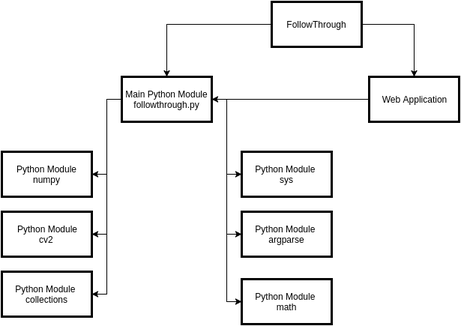
\includegraphics{uses_hierarchy.png}
    \caption{Uses Hierarchy}
    \label{fig:figure1}
\end{figure}


\section{Requirements Traceability}
The chart below explains the connections between the requirements and how they are linked to the functional requirements in the requirements document.\\

\subsection{Traceability Chart}
\begin{table}[h!]
  \centering
  \caption{Traceability Chart}
  \label{tab:table6}
  \begin{tabular}{|p{\dimexpr0.333\textwidth-2\tabcolsep-\arrayrulewidth\relax}
                p{\dimexpr0.333\textwidth-2\tabcolsep-\arrayrulewidth\relax}
                p{\dimexpr0.333\textwidth-2\tabcolsep-\arrayrulewidth\relax}|
              }
    \toprule
    Requirement & Link & Module\\
    \midrule
    3. Store Results & This is needed for the seamless link between website and the on the court interface. & Website and Application\\
    \hline
    5. Upload Data & This is necessary to obtain the data for the on line interface. & Website and Application\\
    \hline
    6. Record Data & This is crucial for the on line interface and general software interface. & Website and Application\\
    \hline
    7. Give Feedback & This is needed for the user to receive real time feedback. & Application\\
    \hline
    8. Access Data & This is also needed for the on line interface portion of the product. & Website\\
    \hline
    9. Retrieve Data & This is also crucial for the on line interface. & Website\\
    \bottomrule
  \end{tabular}
\end{table}

\section{Challenges and Solutions}

\subsection{Challenges}
This sub-section will cover the challenges mentioned in previous documents.
\begin{itemize}
    \item The software needs to successfully track the ball with no cutting.
    \item The hardware has to be safe in its environment.
    \item The software must be able to connect all the hardware together.
    \item The software must be able to upload/update data with no mistakes.
\end{itemize}

\newpage

\subsection{Solutions}
This sub-section will cover the solutions to the aforementioned challenges.
\begin{itemize}
    \item The meanshift algorithm will ensure that the ball is tracked thoroughly and completely within the entire process of running the application.
    \item The hardware will be safely secured on the site where it is being used.
    \item The software and hardware will all be connected through wireless Internet.
    \item The software will upload and update any data to a central server which holds the database for all the data.
\end{itemize}


